\section{Time dilation from vortex dynamics}

We consider an invisible, irrotational superfluid æther with stable topological vortex nodes. Absolute time $t_{\text{abs}}$ flows at a constant rate, while local clocks may experience a lower rate due to pressure gradients and nodal energetics. The Vortex Æther Model assumes that the rate at which time flows in the local frame (near the node) depends on the internal angular frequency $\Omega_k$. In this section, we derive time dilation analogues, inspired by the predictions of general relativity (GR), based solely on pressure and vorticity gradients in the fluid.

\begin{figure}[htbp]
    \centering
    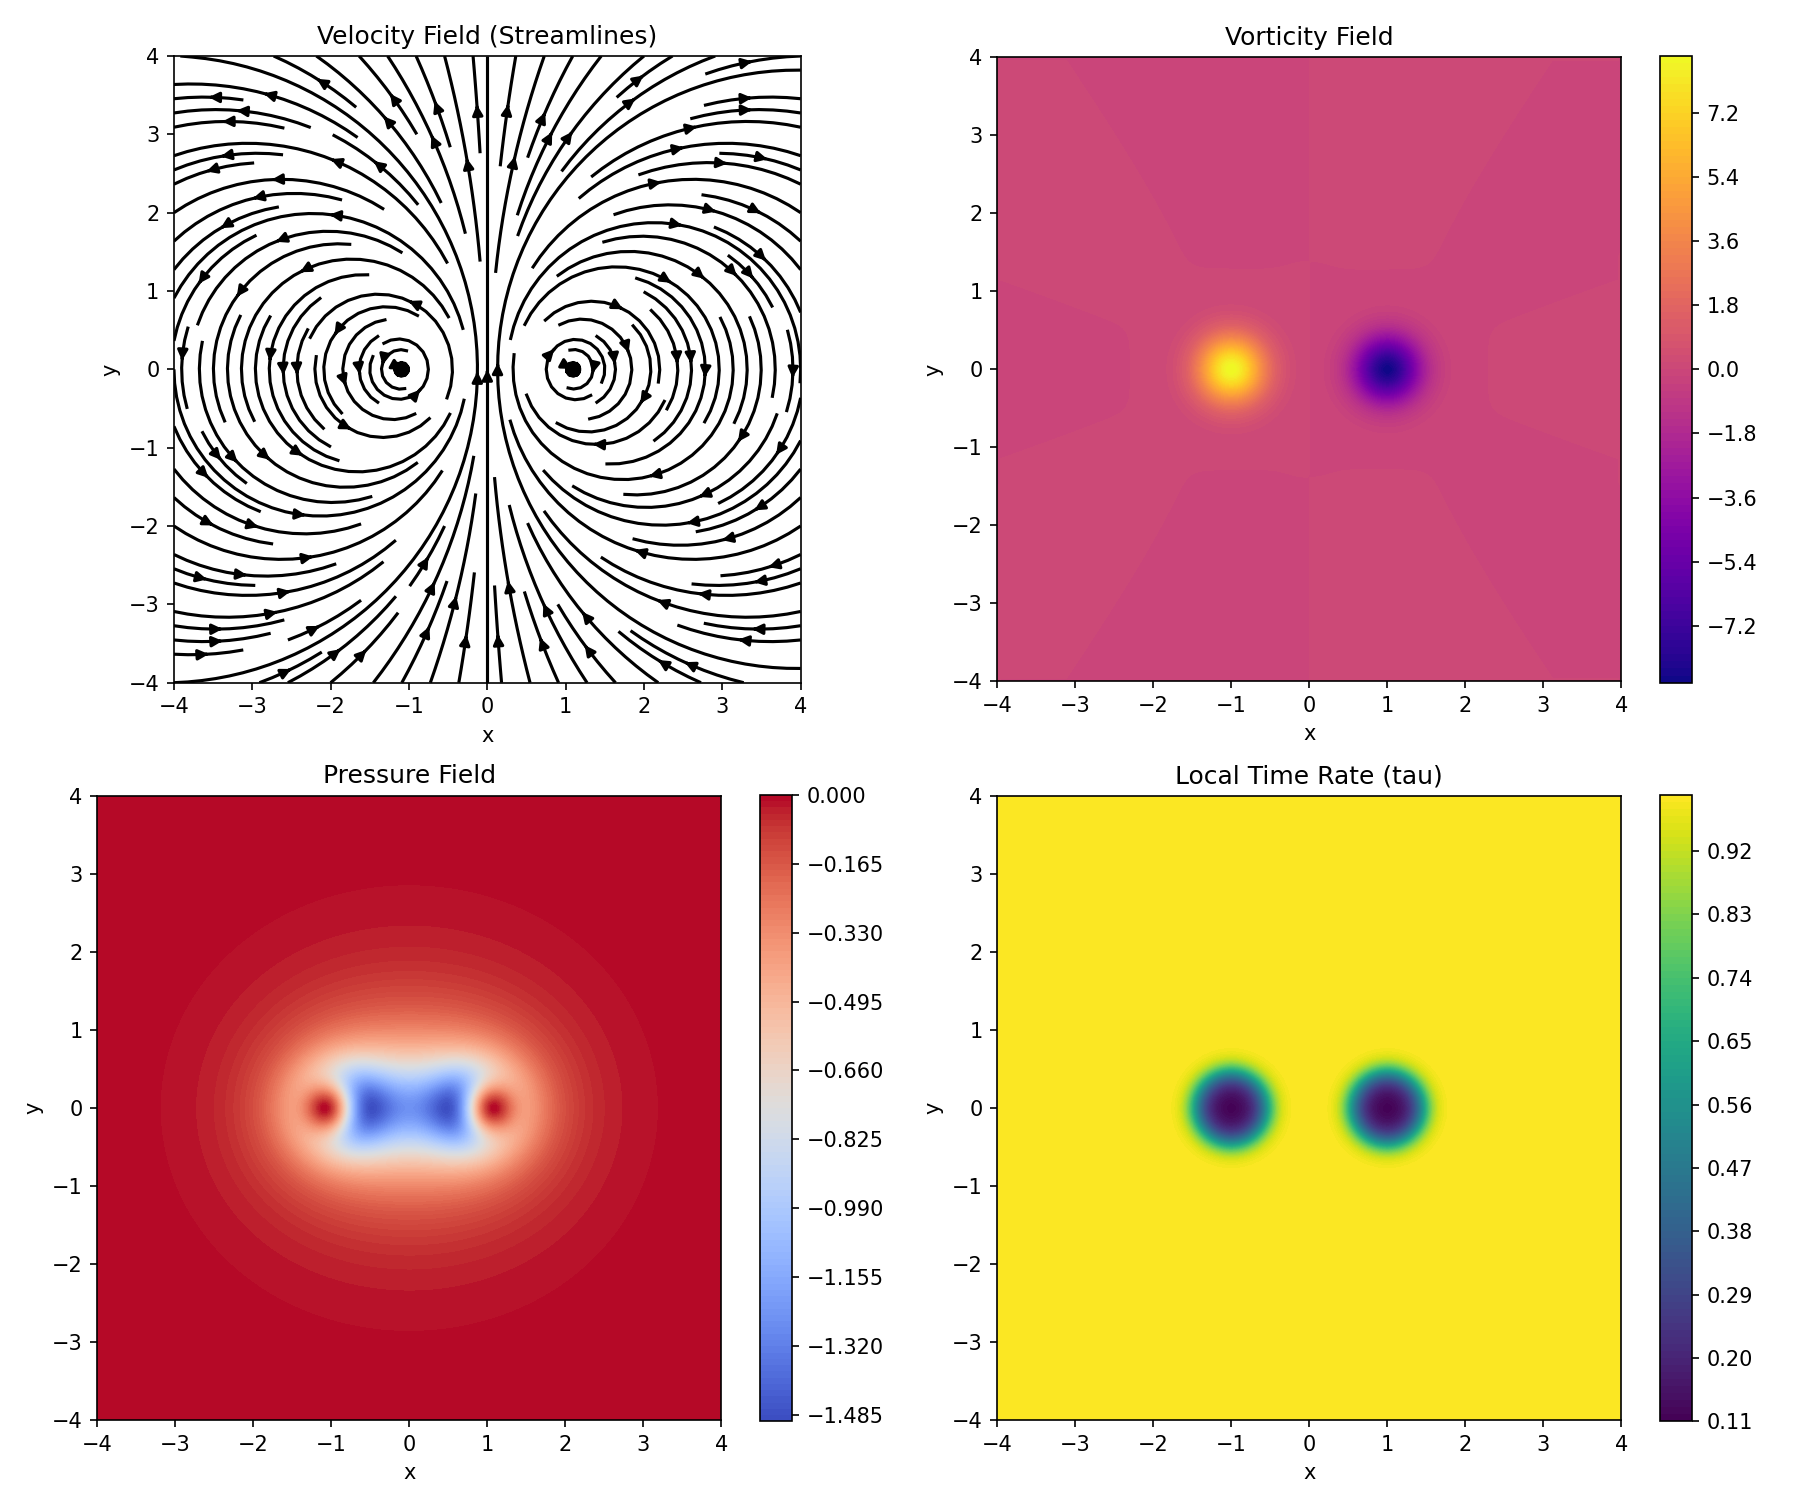
\includegraphics[width=0.85\textwidth]{streamlinesDiPole}
    \caption{Velocity streamlines, vorticity, pressure and local time velocity $\tau$ for a simulated vortex pair. The pressure minimum and the time delay clearly correspond to the regions of high vorticity. This immediately illustrates the central claim of the Æther model: time dilation follows from vortex energetics and pressure reduction.}
    \label{fig:vortexfields}
\end{figure}

In the Vortex Æther Model (VAM), time dilation does not arise from the curvature of spacetime, but from local vortex dynamics. Each particle of matter in VAM is a vortex-node structure whose internal rotation (\textit{swirl}) influences the local clock frequency.

The fundamental link between local vortex velocity and local time measurement follows from the Bernoulli-like relation for pressure reduction in flow fields. The local clock frequency is related to the vortex tangential velocity $v_{\phi}(r)$ by the formula:
\begin{equation}\label{eq:vortex_time_dilation}
\frac{d\tau}{dt} = \sqrt{1 - \frac{v_{\phi}^2(r)}{c^2}}
\end{equation}

Where $v_{\phi}(r)$ is the tangential velocity of the æther medium at distance $r$ from the center of the vortex, and $c$ is the speed of light. This is a direct analogy with the special relativistic velocity-dependent time dilation, but without spacetime curvature and caused solely by local rotation of the æther medium.

\subsection{Derivation from vortex hydrodynamics}

The derivation follows from the Bernoulli principle for an ideal fluid flow, given by:
\begin{equation}\label{eq:Bernoulli}
P + \frac{1}{2}\rho_{\ae} v^2 = \text{constant}
\end{equation}

With vortex flow introduced via vorticity $\vec{\omega} = \nabla \times \vec{v}$, the local pressure reduction relative to the distant environment defines a local time delay. The local vortex velocity is given by:
\begin{equation}\label{eq:tangential_velocity}
v_{\phi}(r) = \frac{\Gamma}{2\pi r} = \frac{\kappa}{r}
\end{equation}

where $\Gamma$ is the circulation constant, and $\kappa$ is the circulation quantum. Substitution of \eqref{eq:tangential_velocity} into \eqref{eq:vortex_time_dilation} gives explicitly:
\begin{equation}\label{eq:vortex_time_explicit}
\frac{d\tau}{dt} = \sqrt{1 - \frac{\kappa^2}{c^2 r^2}}
\end{equation}

This explicitly expresses the time dilation in fundamental vortex parameters.

\subsection{Comparison with general relativity}

For comparison, in general relativity (GR), gravitational time dilation arises from spacetime curvature, expressed by the Schwarzschild metric~\cite{schutz2009first}:
\begin{equation}\label{eq:GRtime}
\frac{d\tau}{dt} = \sqrt{1 - \frac{2GM}{rc^2}}
\end{equation}

The similarities and differences are immediately apparent: GR's gravitational time dilation is related to mass $M$ and gravitational constant $G$, while VAM time dilation is purely hydrodynamic and directly connected to the local rotational velocity of the æther medium via vortex circulation $\kappa$.

\begin{figure}[ht!]
    \centering
    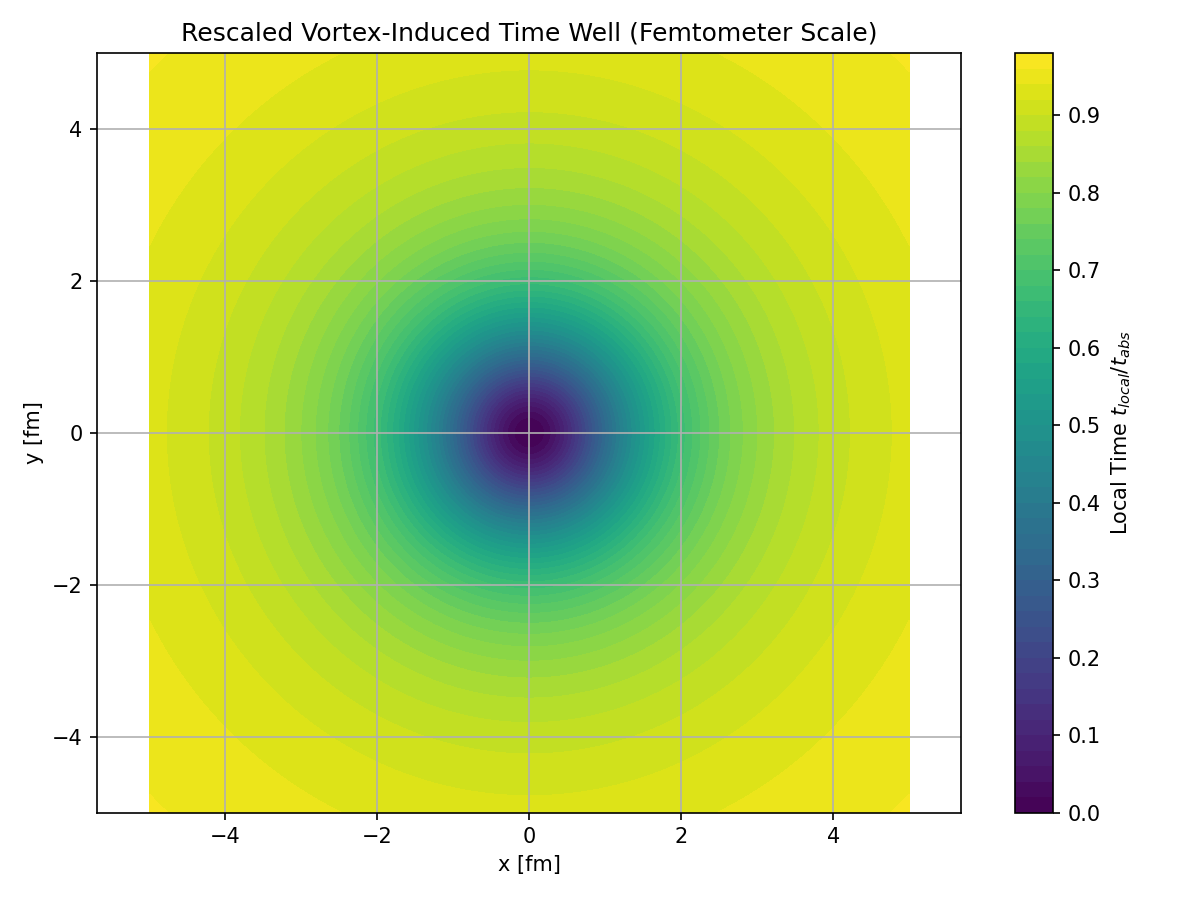
\includegraphics[width=0.7\linewidth]{RadialProfileOfLocalTimeDilation_Vortex-Induced_Time_Well}
    \caption{Comparison of VAM (vortex dynamics) and GR time dilation, as a function of distance to vortex core and Schwarzschild radius.}
    \label{fig:vergelijking_VAMGR}
\end{figure}

In Figure~\ref{fig:vergelijkingVAMGR} we see that VAM time dilation is functionally comparable to GR prediction at sufficient distance. At decreasing distance (near vortex core or Schwarzschild radius) differences arise due to vortex-specific effects and topological node structures.

In summary, the VAM replaces spacetime curvature with eddy dynamics, while preserving measurable time dilation effects consistent with established experimental results such as Hafele–Keating~\cite{hafele1972around}, but from a fundamentally different physical explanation.

For illustration, in Figure~\ref{fig:vergelijkingVAMGR} we explicitly compare VAM and GR for a neutron star with $M = 2\,M_\odot$ and radius $R = 10\,\text{km}$. The differences become clear near the surface of the object, where vortex-specific effects occur.

\begin{figure}[ht!]
    \centering
    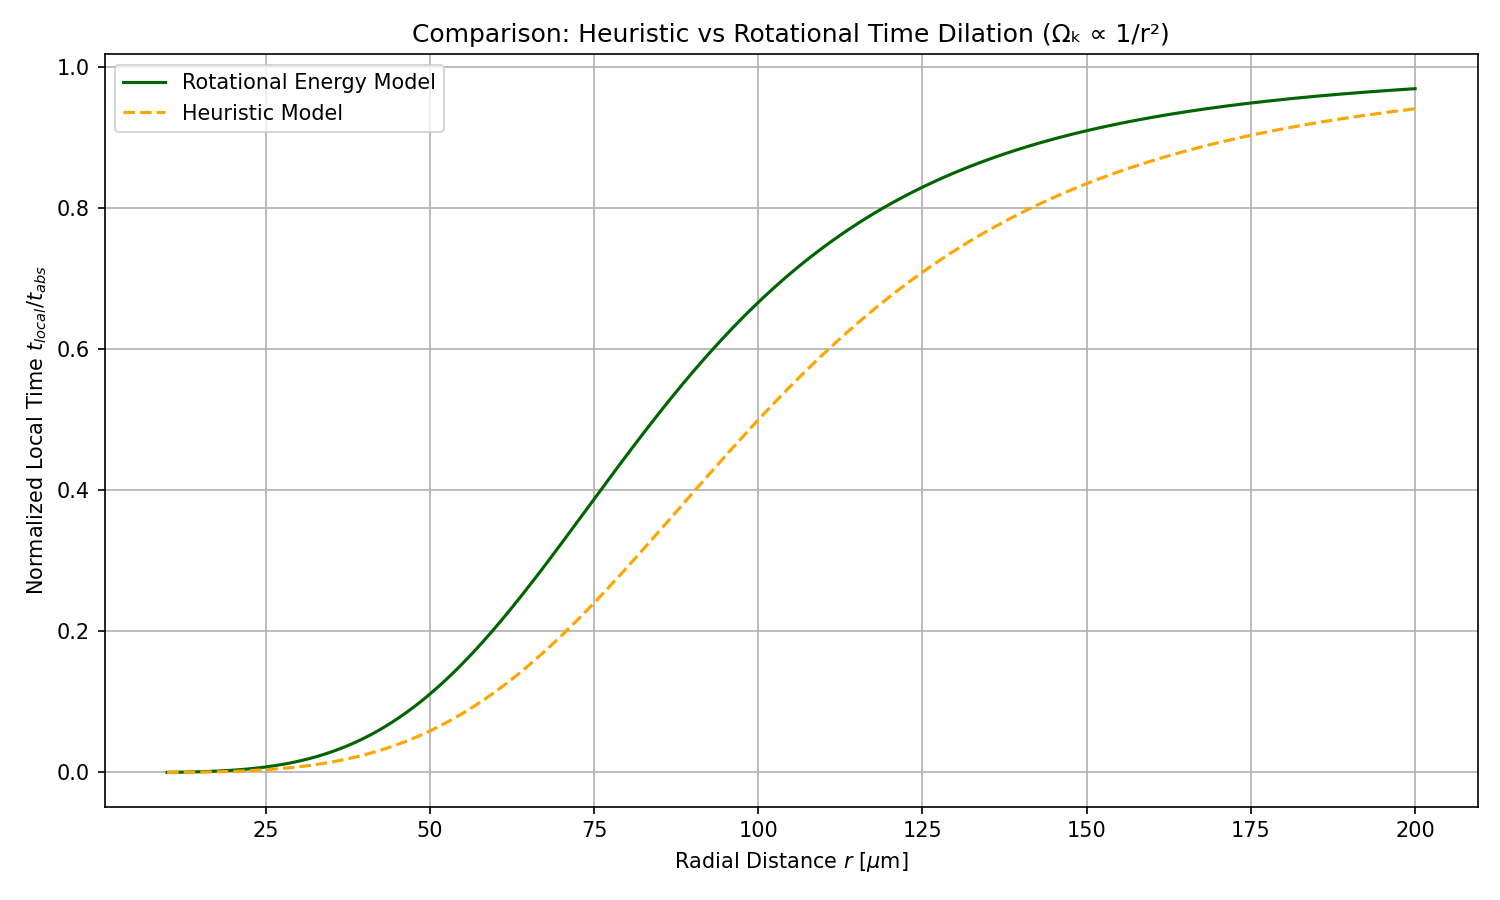
\includegraphics[width=0.7\linewidth]{RotationalVsHeuristicTimeDilation}
    \caption{Difference between VAM and GR time dilation for a neutron star ($2\,M_\odot$, $R=10$ km).}
    \label{fig:comparisonVAMGR}
\end{figure}

\subsection{Interpretation of scale-dependent æther density}

VAM uses a scale-dependent æther density: locally very high ($\sim10^{18}$ kg/m³) for core stability and macroscopically low ($\sim10^{-7}$ kg/m³) to allow inertia-free propagation of interactions. The high density in vortex cores locally enhances the vortex velocity and thus the time dilation significantly, while macroscopically it offers minimal resistance to propagation of effects.

\subsection{Practical implications and experimental testability}

A practical implication of vortex-induced time dilation is that clocks would run measurably slower close to intense vortex fields. This can be tested theoretically with ultra-precise atomic clocks in laboratory vortex experiments, or indirectly via astrophysical observations of pulsars and neutron stars. The Hafele–Keating experiment provides a direct analogy for time dilation due to motion and height differences, which in VAM corresponds to local vortex variations~\cite{hafele1972around}.